\section{Auswertung}
\label{sec:Auswertung}

\subsectin{Ausmessung des Acryl Blocks mittels A-Scan}

Die Ausmessung mittels einer Schieblehre führt zu den Daten, die in Tabelle \ref{fig:mess1} 
dargestellt sind. 

\begin{table}
  \centering
  \caption{Messdaten des Acrylblocks}
  \label{tab:mess1}
  \sisetup{table-format=2.1}
  \begin{tabular}{c c}
  \toprule
  &$Messung \,/\, \si{\centi\meter}$\\
  \midrule 
  Länge  & 15.000\\
  Höhe   &  8.035\\
  Breite &  3.995
  \bottomrule
  \end{tabular}
  \end{table}

Der A-Scan liefert Laufzeiten, die den Ort der Fehlstellen angeben. Bei diesen ist zu beachten, 
dass zunächst die Laufzeit des Koppelmaterial und der Schutzschicht von den Ergebnissen 
subtrahiert werden müssen. Die Schutzschicht hat eine Dicke von $SI{0.2}{\centi\meter}$. 
Aus diesen werden, die Abstände $D_\text{oben}$ der oberen Enden der Fehlstellen zu dem oberen Ende des 
Blocks sowie die Abstände $D_\text{unten}$ der unteren Enden der Fehlstellen zu dem unteren Ende des Blocks 
bestimmt. Für diese Berechnung wird eine Phasengeschwindigkeit in Acryl von $\SI{2730}{\meter\per\second}$ im 
Weg-Zeit-Gesetz verwendet [2]. Zusammen mit der ermittelten Höhe des Blockes ergeben sich die Durchmesser 
der Fehlstellen $D_\text{Loch}$. Diese Werte finden sich in Tabelle ---.

\begin{table}
\centering
\caption{Messdaten des Acrylblocks}
\label{tab:mess1}
\sisetup{table-format=2.1}
\begin{tabular}{c c c c c c}
\toprule
Stelle & $t_1 \,/\, \si{\micro\second}$ & $t_2 \,/\, \si{\micro\second}$ &$D_\text{oben} \,/\, \si{\centi\meter}$&$D_\text{unten} \,/\, \si{\centi\meter}$ & $D_\text{Loch} \,/\, \si{\milli\meter}$\\
\midrule 
3 & 48,5 & 14,1 & 6,25 & 1.56 & 2.25 \\
4 & 42,6 & 19,6 & 5,44 & 2.31 & 2.80\\
5 & 36,6 & 25,1 & 4,63 & 3.06 & 3.48\\
6 & 30,2 & 30,5 & 3,75 & 3.80 & 4.85\\
7 & 24,3 & 36,3 & 2,95 & 4.59 & 4.98\\
8 & 18,6 & 42,0 & 2,17 & 5.37 & 4.98\\
9 & 12,7 & 47,9 & 1,37 & 6.17 & 4.98\\
\bottomrule
\end{tabular}
\end{table}

%\begin{figure}
%  \centering
%  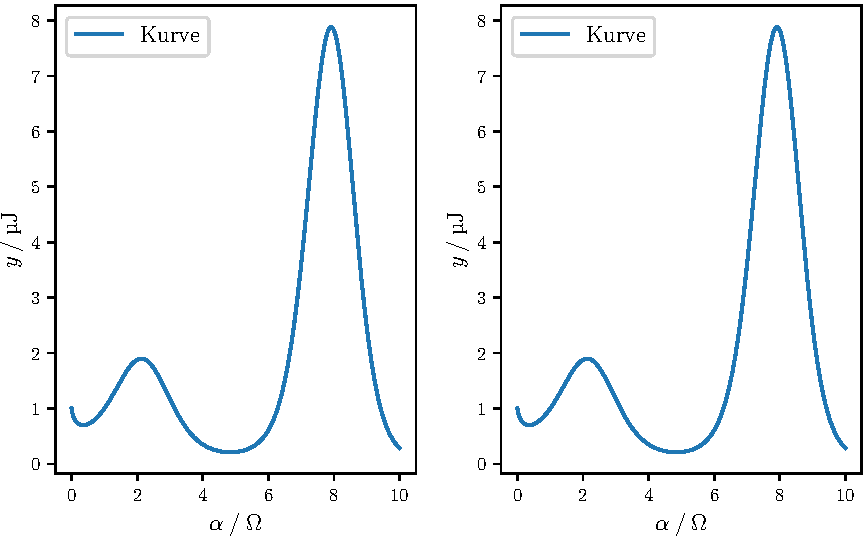
\includegraphics{plot.pdf}
%  \caption{Plot.}
%  \label{fig:plot}
%\end{figure}
